\begin{flushleft}
{\Huge Vinvisor\\}
\end{flushleft}

\vspace{2cm}
\begin{center}
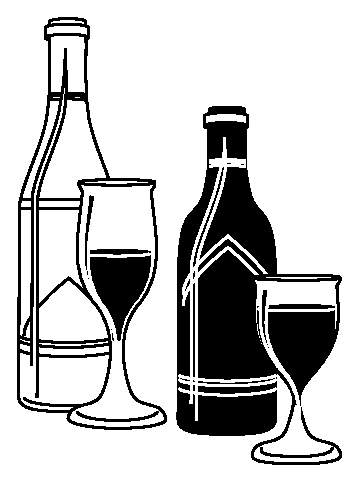
\includegraphics[width=6cm]{bilder/63.eps}

{\Large
\vspace{1cm}
In vino veritas}
\end{center}

\newpage
\begin{song}{Bordeaux, Bordeaux}{bordeaux}
\mel{I sommarens soliga dagar}
\begin{vers}
Jag minns än i dag hur min fader\\
kom hem i från staden så glader.\\
Han rada' upp flaskor i rader,\\
och sade nöjd som så: Bordeaux, Bordeaux!\\
Han drack ett glas, kom i extas,\\
och sedan blev det stort kalas.\\
Och vi små glin, ja vi drack vin,\\
som första klassens fyllesvin,\\
och vi dansade runt där på bordet\\
och skrek så vi blev blå:\\
Bordeaux, Bordeaux!\\
\end{vers}
\end{song}

\begin{song}{Nattvarden}{nattvarden}
\mel{We are all the winners}

\begin{vers}
Snabba på med vinet\\
söla inte präst\\
Strunta i oblaten, nu så är det fest\\
Skynda, fram med kalken\\
skit i orgelbrus och sång\\
Nu så ska vi ägna oss åt Nattvard dagen lång\\ 
\end{vers}
\end{song}

\newpage

\begin{song}{Vinet}{vinet}
\mel{Rullan går}
\begin{vers}
Vinet är ett märkligt ting,\\
märkligt ting, märkligt ting.\\
Bäst man känner ingenting,\\
ingenting, ingenting.\\
Vips man blir rätt yr i hatten,\\
dagen efter älskar vatten.\\
Men vad gör väl det ikväll?\\
Glaset höj, gutår och häll!\\
\end{vers}
\end{song}

\begin{song}{Sudda sudda}{suddasudda}
\begin{vers}
Sudda, sudda, sudda, sudda bort din sura min.\\
Med fyra jättestora bamseklunkar ädelt vin.\\
Munnen den skall sjunga och va' gla'.\\
För att den skall bli som den skall va'.\\
Vad häller du då bak det dolda flinet?\\
Vinet som suddar, suddar bort din sura min.\\
\end{vers}
\end{song}

\newpage

\begin{song}{Nu grönskar det}{nugronskardet}
\mel{Bondekantat}
\begin{vers}
Nu grönskar det i dalens famn, \\
nu doftar äng och lid.\\
Kom med, kom med på vandringsfärd\\
i vårens glada tid!\\
Var dag är som en gyllne skål,\\
till brädden fylld med vin.\\
så drick, min vän, drick sol och doft,\\
ty dagen den är din.\\
\end{vers}
\begin{vers}
Långt bort från stadens gråa hus \\
vi glatt vår kosa styr.\\
Och följer vägens vita band\\
mot ljusa äventyr.\\
Med öppna ögon låt oss se\\
på livets rikedom\\
som gror och sjuder överallt\\
där våren går i blom!\\
\end{vers}
\end{song}

\newpage

\begin{song}{Feta fransyskor}{fetafransyskor}
\mel{Marsche militaire}
\begin{vers}
Feta fransyskor som svettas om fötterna\\
de trampar druvor som sedan skall jäsas till vin\\
Transpirationen viktig e'\\
ty den ger fin bouquet\\
Vårtor och svampar följer me',\\
men vad gör väl de'?\\
\end{vers}
\begin{vers}
För...\\
\end{vers}
\begin{vers}
Vi vill ha vin, vill ha vin, vill ha mera vin\\
även om följderna bli att vi må lida pin\\
\textit{Flickor:}   Flaskan och glaset gått i sin.\\
\textit{Pojkar:}    Hit med vin, mera vin!\\
\textit{Flickor:}   Tror ni att vi är fyllesvin?\\
\end{vers}
\begin{vers}
JA! (Fast större)\\
\end{vers}
\end{song}

\newpage

\begin{song}{Undulaten}{undulaten}
\mel{Med en enkel tulpan}

\begin{vers}
Jag är en liten undulat\\
som får så dåligt med mat\\
för dom jag bor hos\\
ja dom jag bor hos\\
dom är så snåla.\\
Jag får ju fisk varenda dag\\
men det vill jag inte ha\\
jag vill ha rödvin\\
jag vill ha rödvin och gorgonzola\\
\end{vers}
\end{song}


\begin{song}{Ta ett glas}{taettglas}
\mel{Oh Tannenbaum}

\begin{vers}
Oh, ta ett glas,\\
Oh, ta ett glas.\\
Ty vinet för oss samman.\\
Och den som inget glas vill ha,\\
han sjunger och är lika gla'.\\
Men ta ett glas,\\
ja ta ett glas,\\
för livets fröjd och gamman.\\
\end{vers}
\end{song}

\newpage

\begin{song}{Vårvinets lov}{varvinetslov}
\mel{I sommarens soliga dagar}

\begin{vers}
Se, vinet det glimmar i glasen,\\
av vin blir det glatt på kalasen.\\
Sopranen, tenoren och basen\\
vid Bacchi hov\\
vill sjunga vinets lov.\\
Därför ej dröj - pokalen höj\\
och dig med druvans saft förnöj.\\
En nektar som vi tycker om\\
och återverkar småningom.\\
I vårdagars roliga stunder\\
ett glatt och fylligt vin är melodin!\\ 
\end{vers}
\end{song}

\begin{song}{Elysisk längtan}{elysisklangtan}
\mel{An die Freude}
\begin{vers}
Aftonrodnan svalka sprider\\
skymningen sig sänker fin\\
och likt dimridåer sprider\\
doften av det rena vin\\
\end{vers}
\begin{vers}
//: Låt det hjälpa mig till att segla\\
rakt in i rusets röda tröst\\
natten flyr på gryningsvingar\\
värmen flammar i mitt bröst ://\\
\end{vers} 
\end{song}

\newpage

\begin{song}{Så länge rösten är mild}{salangerosten}
\mel{Så länge skutan kan gå}
\begin{vers}
Så länge rösten är mild\\
så länge ingen är vild\\
så länge spegeln på väggen\\
ger halvskaplig bild\\
Så länge alla kan stå\\
så länge alla kan gå\\
så länge alla kan tralla så fyller vi på\\
\end{vers}
\begin{vers}
För vem har sagt att\\
just du kom med storken\\
för att bli glad\\
av att lukta på korken\\
Så till kvinns och till mans\\
vi höjer bägar'n med glans\\
och låter vinet gå ner\\
i en yrande dans\\
\end{vers}
\end{song}


